\documentclass[10pt,twocolumn]{article}
\usepackage{amsmath}
\usepackage{amsfonts}
\usepackage{amssymb}

\usepackage{epsfig}
\title{A Framework for Personalized Photograph Quality Assessment}
\author{
K. Armin Samii \\
ksamii@ucsc.edu
\and
Uliana Popov \\
uliana@soe.ucsc.edu}
\date{May 13, 2011}

\begin{document}
\maketitle
\begin{abstract}
Photograph quality assessment can help aid home users in managing their personal collections in several ways, including deleting low-quality images and browsing for high quality images. Recent research has aimed to automatically rate image quality, but such methods are far from perfect and progress is slow. In this paper, we propose a framework for quickly developing and testing new features to accelerate the progress of this research. We have two types of features: \textit{high-level features} are subjective qualities which humans can easily answer; \textit{low-level features} are objective calculations which are produced algorithmically. We use machine learning techniques to learn how each of these relate to image quality. Our model allows for a developer to easily train new features (both low-level and high-level), and for an end-user to personalize which high-level features are important.

%First, we find how each high-level feature corresponds to overall image quality, allowing for user-adjusted preferences. Next, we find how the low-level features corresponds to each high-level feature. Finally, we allow both the low-level and high-level features to be dynamically adjusted by the developer with ease. We use basic Human Computation to obtain a ground truth.


\end{abstract}

\section{Problem Statement}
A photographer wishes to automatically rate his pictures based on personal preferences. There are several works dedicated to solving this problem. To accelerate research in the area, we need to develop a framework for developers (researchers) to quickly train new features extracted from photographs.

There are two audiences we are trying to serve in this work: the photographer using the application, and the developer producing the application. In other words, we want to make it as easy as possible for the developer to serve the photographer.

To do so, we first want to allow the photographer to choose which features are important to her personally.
%However, many of the features extracted from photographs are highly algorithmic and make little intuitive sense (e.g. "Blurriness" is more intuitive than "Average edge width"). We call these \textit{low level features}. These low level features are hidden from the user and instead, the user is shown \textit{high level features}, which may contain several low-level features.
Second, we want the developer of the quality-assessment application to be able to add new features with ease.

We make the distinction between \textit{low-level features} (ones that are computed, such as average edge width) and \textit{high-level features} (ones that are solely for human interpretation, such as blurriness, and that may consist of several low-level features). 

Figure \ref{fig:flowchart} visualizes these ideas. We will describe them in detail below to make the specific purpose of this paper more clear.

\begin{figure*}[t!]
    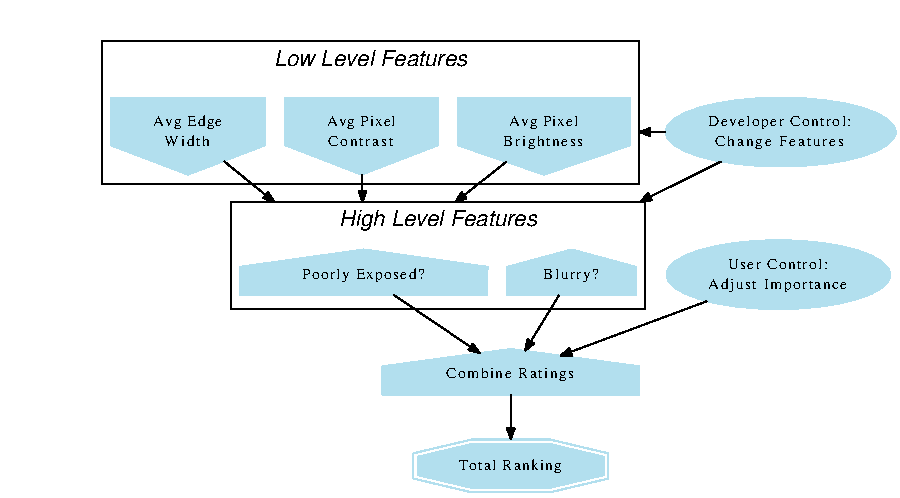
\epsfig{file=mlflowchart.pdf,width=16cm}
  \caption{An example flowchart. Here, the application computes three low-level features. All three influence the two high-level features: blurriness and exposure. The developer controls which features are present. The photographer decides how to weight each high-level feature.}
  \label{fig:flowchart}
\end{figure*}

\subsection{Abstraction from the Photographer}
\label{abstraction}
This problem boils down to the following two questions:

\begin{enumerate}
\item \textbf{How important is each high-level feature to the overall rating of a photograph?}

This question is relevant to the photographer. As an example:

%Photographers Penny and Quinn want to automatically rate their photographs so they can ignore those with low ratings and save some time when browsing their collections.
Photographer Penny takes pictures at concerts so she doesn't mind slightly underexposed images. Penny will decrease the default weight on the high-level "exposure" feature.

\item \textbf{How does each low-level feature affect the ranking of a high-level feature?}

This  question is relevant to the developer. As an example:

Programmer Pete calculates three low-level features per image: average width of edges, average pixel contrast, and average pixel brightness. He wants to use these low-level features to obtain a rating for the amount of blur in an image.
\end{enumerate}

\subsection{Ease of progress for the developer}
\label{easeofprogramming}
Say Programmer Pete finds a new way to measure blur levels in an image. He should be able to insert this feature into the program with ease. Because of the abstraction above, the photographer would be unaware of any changes.

Instead, if Pete realizes that some new high-level feature is relevant to overall image quality (say, the saturation of the image), then he will want to see just how much saturation is relevant to image quality. The end-user photographers will be aware of this new change, and can adjust the high-level weights accordingly.

\section{Introduction}
To solve the problem presented, one might try to directly train low-level features to rate image quality. However, photograph quality is highly subjective and this approach does not allow a photographer to personalize the importance of each feature.

So instead, one might try to compute high-level features directly and allow the photographer to personalize the importance this way. However, this method risks using a poor algorithm to calculate a high-level feature, and thus sacrifices accuracy.

We thus propose a method which separately trains low-level and high-level features. This method allows (1) the photographer to personalize each feature's importance, and (2) the programmer to choose the best possible method for rating each high-level feature on an image.

Further, the programmer utilizing our framework will decide which features to include. We allow the programmer to dynamically modify the features by retraining on a held-out test set.

Training our data is broken down into two steps. First is determining the importance of each high-level feature. To do so, we need to see how much influence each high-level feature has on overall image quality. (We describe how we obtain this data in Section \ref{turkdata}.) Second, we determine how much influence each low-level feature has each high-level feature. The learning methods we use are described in detail in Section \ref{methods}.

\section{Related Work}
Tong and Chang\cite{Tong:2001:SVM:500141.500159} use Support Vector Machines to search a database of images quickly by choosing images that are visually similar, which abstracts the features from the user completely.

The Personalized Photograph Ranking and Selection System\cite{Yeh:2010:PPR:1873951.1873963} computes high-level features directly and uses ListNet\cite{Cao:2007:LRP:1273496.1273513} to find a ranking. However, this does not allow for the training of several low-level features to produce a single high-level feature, which can increase the overall accuracy.

\section{Data}

There are two sets of data used, both of which are learned independently.

\subsection{User-Produced Data}
\label{turkdata}
The initial set of data was produced by giving Turkers a simple statement for each high level feature, and asking if they agreed. Our primary, ground-truth statement for each image is:

``This image is high quality.''

We present this to five Turkers and ask them to choose one of three options, each of which corresponds to some number of points gained for each high-level feature:

\begin{itemize}
\item ``Agree'' (+1 point)
\item ``Neutral'' (+.5 points)
\item ``Disagree'' (+0 points)
\end{itemize}
The points are then averaged across the five Turkers' responses to come up with a final score.

We repeat this process for each high level feature, with statements such as ``This image is in focus'' and ``This image is well-exposed.'' The data then looks like:

\resizebox{7.5cm}{!}{
\begin{tabular}[t]{| c | c | c | c | l | }
 \hline
 & High Quality & In focus & Well exposed & \ldots \\ 
 \hline
Image 1 & .5 & .25 & 1 & \ldots \\ 
 \hline
\vdots & \vdots & \vdots & \vdots & $\ddots$ \\
 \hline
\end{tabular}
}

This data is used in a Logistic Regression to relate each high-level feature to the first statement (``This image is high-quality'').

\subsection{Application-produced data}
The application produces numbers for each high-level feature.

\section{Training Methods}
\label{methods}

First, we use a logistic regression to calculate weights on which high-level features appeal to humans in photographs. We then use Support Vector Machines (SVMs) to match low-level features extracted algorithmically to high-level features. For example, the high level feature of "exposure" has more weight than "blur," and the low-level feature of "average pixel color" affects "exposure" more than it affects "blur." We then allow the weights of high-level features to be adjusted by users to allow personalization. The result is a rating of an image based on the base high-level weights and the user's individual preferences.

We keep a held-out test set to recalculate parameters when the developer adds a feature. When a new high-level feature is added, we ask Amazon Mechanical Turk\footnote{http://www.mturk.com} users ("Turkers") to rank an image based on that feature. When a low-level feature is added, the parameters of each of the SVMs are updated.


\section{Progress thus far [informal]}
So far, we have gathered several hundred data points for two high-level features. We have increased the speed of previously written code to allow for several dozen images to be processed in a minute (as opposed to about 2 minutes per image previously).

We have implemented Support Vector Machines into our code and it is working on a small test set. We have a mostly-completed framework for dynamically changing high- and low-level features. No progress has been made on determining the weights of each high-level feature (for logistic regression).

We should note that we talk about our work as if the project were completed. It is not.


\section{Results [informal]}
We have a test set of several hundred images that we expect our application will return a high number on, and another test set of several hundred blurry images. We do not plan on using these for training because they do not match the rest of our data (they were not obtained from Turk), but we can ensure that after training we received better results (and we can measure based on how much better we perform). This does not take into account user preferences or ease of use of our framework.

\bibliographystyle{plain}
\bibliography{README_BIB}

\end{document}
